\documentclass{lutmscthesis}[2010/09/22]

\usepackage[latin1]{inputenc}
\usepackage[T1]{fontenc}
\usepackage[english,finnish]{babel}

\usepackage{times}

\usepackage{setspace}
\usepackage{verbatim}
\usepackage[intlimits]{amsmath}

% Ensure figure captions are below and table captions are above the content.
\usepackage{float}
\floatstyle{plain}\restylefloat{figure}
\floatstyle{plaintop}\restylefloat{table}

\usepackage[pdfborder={0 0 0}]{hyperref}


\graphicspath{{resources/images/}}                % Graphics search path

\newcommand{\vect}[1]{\boldsymbol{#1}}
\newcommand{\matr}[1]{\boldsymbol{#1}}
\newcommand{\diag}[1]{\mathrm{diag}(#1)}
\newcommand{\iprod}[1]{\left\langle #1 \right\rangle}
\newcommand{\me}{\mathrm{e}}
\newcommand{\mi}{\mathrm{i}}
\newcommand{\md}{\mathrm{d}}
\newcommand{\sse}{{}} %\mathrm{SSE}}
\newcommand{\trace}{\mathrm{Tr}\:}
\newcommand{\frp}[2]{{}^\mathrm{#1}\vect{#2}}
\newcommand{\frs}[3]{{}^\mathrm{#1}#2_\mathrm{#3}}
\newcommand{\frv}[3]{{}^\mathrm{#1}\vect{#2}_\mathrm{#3}}
\newcommand{\frm}[3]{{}^\mathrm{#1}\matr{#2}_\mathrm{#3}}
\newcommand{\colvec}[2]{\genfrac{[}{]}{0pt}{1}{#1}{#2}}
\newcommand{\relphantom}[1]{\mathrel{\phantom{#1}}}

% Tables
\usepackage{array}
\usepackage{multirow}
\newcolumntype{L}[1]{>{\raggedright\let\newline\\\arraybackslash\hspace{0pt}}m{#1}}
\newcolumntype{C}[1]{>{\centering\let\newline\\\arraybackslash\hspace{0pt}}m{#1}}
\newcolumntype{R}[1]{>{\raggedleft\let\newline\\\arraybackslash\hspace{0pt}}m{#1}}

% Code
\usepackage{listings}
\usepackage{xcolor}
\renewcommand{\lstlistingname}{Listing}

\lstset{frame=single,
  language=Python,
  aboveskip=10mm,
  belowskip=0mm,
  captionpos=b,
  basicstyle={\small\ttfamily},
  numbers=none,
  breaklines=false,
  breakatwhitespace=true,
  framexleftmargin=6pt,
  framexrightmargin=6pt,
  framextopmargin=4pt,
  framexbottommargin=4pt
}


% Thesis information
\title{Overview of Machine Vision Applications in Waste Recycling}
\author{Tikhon Belousko}
\Major{Degree Program in Intelligent Computing}
\Faculty{School of Engineering Science}
\Doctype{}
\Keywords{visual inspection, computer vision, machine vision, recycling}
\Supervisor{Leena Ikonen D.Sc. (Tech.)}
\Examiner{Leena Ikonen D.Sc. (Tech.)}
\Year{2016}
\addtostats{, 4 figures, 2 tables, 3 code listings}


% ---
% Document
% ---
\begin{document}
\selectlanguage{english}


% ---
% Title
% ---
\maketitle
\newpage


% ---
% Abstract
% ---
\begin{abstract}

This project involves discovering how machine vision techniques are applied
to the different aspects of sorting and recycling waste. The goal is to shed
a light on the main algorithms used for inspecting many kinds of materials such
as plastic, paper, glass and metal. This has been done by analysis of different
types of scientific articles devoted to the use of machine vision in area of
recycling. It was revealed that there are many techniques and algorithm of
pattern recognition and image analysis used for detecting different types
of waste that could be recycled. It has been shown that machine vision
could significantly improve the process of sorting and make recycling
more effective and easier.

\end{abstract}

% ---
% Table of Contents
% ---
% 1 Table of Contents
% 1. Contents
% 2. Abstract
% 3. Introduction
% 4. Sorting systems of recyclable materials
% 5. Plastic bottles recycling
% 6. Paper Recycling
% 7. Metal Recycling
% 8. Conclusion
% 9. Reference

\renewcommand\refname{REFERENCES}
\renewcommand\contentsname{CONTENTS}
% \pagestyle{masters}
\newpage

\tableofcontents

% ---
% Sorting systems of recyclable materials
% ---
\section{ INTRODUCTION }
\setlength{\parskip}{3ex}

\subsection{ Background }
In recent years, there have been many papers describing
machine vision systems for sorting different kinds
of recyclable materials. Earlier, people were only
able to perform manual sorting, but with
development of pattern recognition and intelligence
techniques the automated sorting started to prevail
in industry. There is considerable variety of the
articles and other sources describing different
algorithms and systems for automatic sorting. Moreover,
usually each article concentrates only on only one
type of waste. For example, the process of sorting
plastic bottles is described in~\cite{Wahab:2006}, the
separation of grades of paper is outlined
in~\cite{Rahman:2009}. However, there not too many
sources which allow to understand what are common
methods for all of the materials, where
you could better understand and analyze how machine
vision can be used to overcome the problem
of waste sorting.

\subsection{ Objectives and Delimitations }
The aim of this paper is to generalize methods and
techniques commonly used for separation of different
kinds of recyclable materials. The overview
is done by analysis of articles describing
systems for sorting plastic and paper waste. The
performance of the suggested systems were also
investigated. It was revealed that most of
the systems include camera sensors. The images
of the objects are preprocessed, and
after feature extraction there are pattern
recognition methods are applied.

\subsection{ Structure of the Report }
The paper is divided into two main sections. The first part
is devoted to plastic recycling. In this part we present
the ideas and algorithm used for sorting two types of resin,
namely PET and non-PET. The second section describes
state of affairs in paper sorting. In this part
we report a method for sorting three kinds of paper:
Old Corrugated Cardboard, Old News Paper and White Paper.



% ---
% Sorting systems of recyclable materials
% ---
\section{ SORTING SYSTEMS OF RECYCLABLE MATERIALS }
\subsection{ Plastic Recycling }

One of the common problem of recycling is separation and recycling
of plastic recycling and techniques
of machine vision have takes significant part in this
process. The most common systems are based on optical
sensors, X-Ray and Near Infrared cameras. Although
these methods show effectiveness, they can be too
expensive and redundant for facilities with low and
high throughput. The idea to overcome this issue
is presented in this section based on ideas from~\cite{Wahab:2006}.


\subsubsection*{ Modern Technologies of Plastic Recycling }

Plastic materials are very lightweight and can be used to
contain many different kinds of liquids or utilized as packaging.
Usually, plastic is divided in several categories of resins, the most common
ones are PET, HDPE, LDPE, PVC, PP and PS, as can bee seen from Table \ref{tab:resin_types}.
Some of this types have various kinds of recyclable applications.
Generally, there are two ways of sorting plastic: manual sorting and
automated sorting. Due to very high cost and small efficiency, companies are
concerned of automating this process. Noteworthy, that for proper recycling process
types resins should not be mixed, otherwise it can lead to
emission of hydrochloric gases.

\begin{table}[hpt]
\begin{center}
\caption{Plastic bottle recycle code system and
         material~\cite{Wahab:2006}.\label{tab:resin_types}}
{\renewcommand{\arraystretch}{2}
\begin{tabular}{C{2cm} | l | C{2cm} | l}

\textbf{Code System} & \textbf{Material} & \textbf{Code System} & \textbf{Material} \\ \hline

% \begin{minipage}{.3\textwidth}
\raisebox{-5mm}{
\includegraphics[width=10mm, height=10mm]{rtype1}}
& 1-PETE Polyethylene terephthalate &
\raisebox{-5mm}{
\includegraphics[width=10mm, height=10mm]{rtype5}}
& 5-PP Polypropylene \\

\raisebox{-5mm}{
\includegraphics[width=10mm, height=10mm]{rtype2}}
& 2-HDPE High-density polyethylene &
\raisebox{-5mm}{
\includegraphics[width=10mm, height=10mm]{rtype6}}
& 6-PS Polystyrene \\

\raisebox{-5mm}{
\includegraphics[width=10mm, height=10mm]{rtype3}}
& 3-PVC Polyvinyl chloride &
\raisebox{-5mm}{
\includegraphics[width=10mm, height=10mm]{rtype7}}
& 7-O Other \\

\raisebox{-5mm}{
\includegraphics[width=10mm, height=10mm]{rtype4}}
& 4-LDPE Low-density polyethylene &
& \\

\end{tabular}}
\end{center}
\end{table}


Manual sorting relies on workers who are walking along the
conveyor belt, picking up bottles of different types and
putting them in different containers. However, method turned
out to be not effective for facilities with high throughput.
Also, it was revealed that workers tend to make mistakes
in course of sorting.

Automated sorting utilizes detection systems which are build
using modern machine vision methods to separate plastic by type,
shape or color. Sorting can be divided on bottle sorting (macro-sorting)
and flake sorting (micro-sorting). The second type is performed on granules
and can process considerable amounts of plastic mass.

Although micros-sorting is starting to gain
popularity in recycling area, whole-bottle sorting
is still prevails in industry. During macro-sorting
process bottles are sorted in different containers
using information about resin type, size or color.
The common systems involved are usually optical, using
X-Ray or Near Infrared signals (NIR).

Camera systems that operate in visible spectrum
can be used to separate bottles by color, although for
sorting of bottles of the same color black and white
camera can be utilized. Modern NIR systems
allow to separate even translucent colored materials.
Moreover, each resin type absorbs only specific wavelengths
emitted by NIR and after that transmits particular signal
to sensor. Thus, NIR can be utilized to effectively
process different type of plastic. The important property
of NIR is that it works correctly even if plastic surface
is contaminated with labels. On the other hand, if bottles
are placed too dense and overlap each other, it can lower
the positive effect. Hence, to make system reliable
bottles should be processed one by one. PVC plastic can
be identified using X-Ray technology, although it requires
registration and should satisfy norms of Occupational Safety
and Health Administration.

Since 1989 the development of automatic plastic sorting systems
has started and just in two years one introduced a system for separating
PVC resin from PETA. It was a starting point, when the problem
of the recycling of the materials got more attention.

Modern automated systems tend to be rather efficient, although
quite often it requires considerable amount of scientific and
technological investments. Because of this reason it may not
be suitable for small or medium size manufacturers. Considering this
issue the authors of~\cite{Wahab:2006} propose imaging systems
that allows separating materials in two classes: PET and non-PET
resin types. The first type is normally used for storing
juices, mineral water and other kinds of drinks while
second type is mostly appropriate for storing chemical
liquids.

\subsubsection*{ Proposed System Description }
Two main aspects which are equally important for any sorting
facility: detection system and mechanism for handling material.
Moreover, for both micro-sorting and macro-sorting
the proper managing of feed stream. Hopper, conveyor belt, the ejector
and the collecting bins make up the handling system,
the detection system is implemented using of machine vision.
The whole scheme of the system is shown on
Figure~\ref{afig:scheme_plastic}.

\begin{figure}[htp]
  {\par\centering
  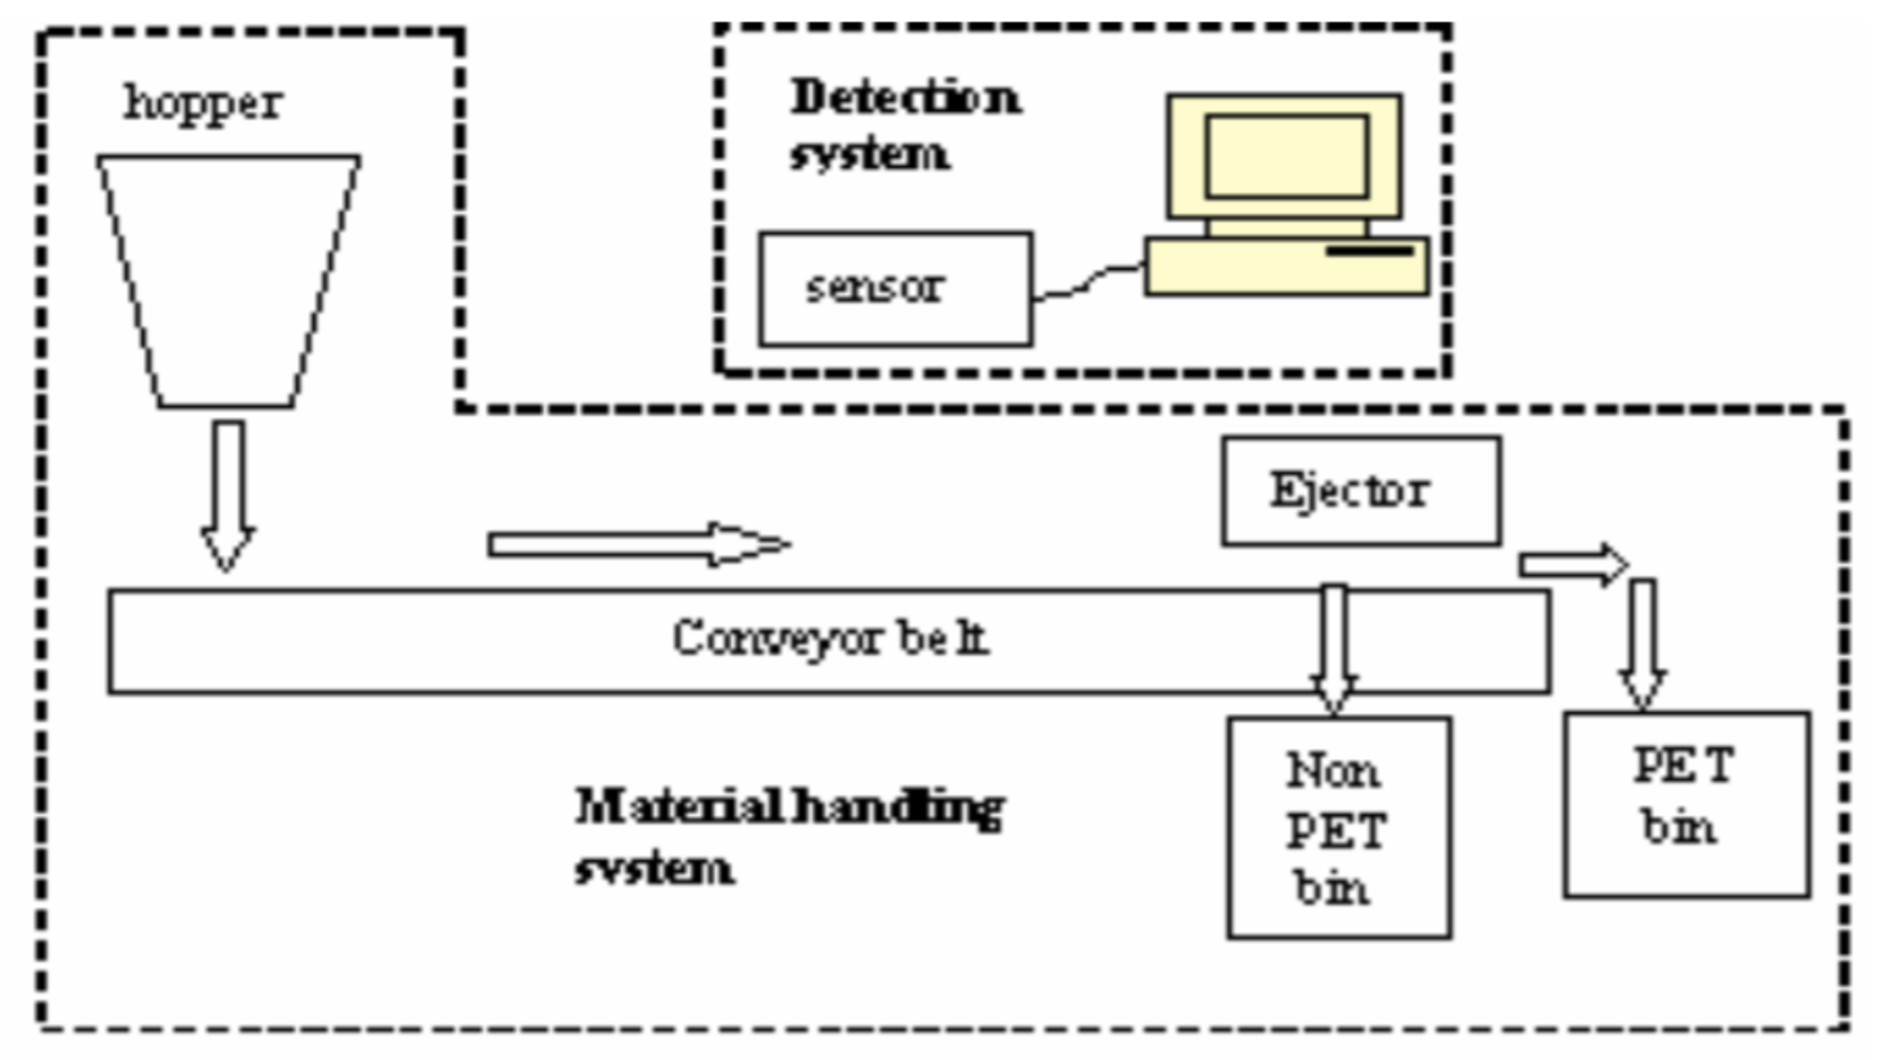
\includegraphics[width=0.60\textwidth]{scheme-plastic}
  \par}
  \caption{A diagrammatic illustration of the automated sorting system~\cite{Wahab:2006}.}
  \label{afig:scheme_plastic}
\end{figure}

The sorting process can be described as follows, first
image is digitalized using internal camera mechanisms.
Next, digital image is going through pre-processing
where it adjusts to particular task, applies filters
and removes defects. After that starts process
of feature extraction which leads classification.

On the pre-processing step image is converting
to binary format using thresholding. The next step is
the usage of morphological operations for
edge detection. The most known morphological operations
are erosion and dilation. The combination of these
two can help to avoid discontinuity in shapes
on image. The output of this process is black-white
image of the same size.

The pre-processed image is further analyzed and
goes as an input to feature extractor which converts
given image to small set of particular features. In presented
work main parameters for extraction were color and
shape of bottles.

Boundary or contour-based, region or area based and skeleton based
are three main approaches for shape representation.
In this system, authors have chosen the first method
and implemented it using Freeman Chain Codes introduced
in 1961 by Herbert Freeman.

For the classification task authors used wide range of different
methods. The first option were to measure Euclidean distance between
image being processed and set of images from stored
dataset. This method has been characterized as reliable
even in case of bottles with identical shapes. Also,
authors considered several artificial neural networks,
utilizing sizes of shapes in pixels. In addition,
the perimeter in polar coordinates was chosen
as a input for trained neural network. The output
of each method were the value which represented
the probability of belonging to particular class. Hence, the
output of pattern recognition technique with highest quality
can be taken as final answer to classification.

\subsubsection*{ Results }

The system was tested and proved its efficiency. Thus,
at least 80\% of the bottles were classified correctly
in poor lightning conditions. In contrast, using
appropriate lightning environment the system reaches
5\% error rate utilizing combination of all presented
algorithms. The advantage of developed system is that
it can be used on facilities with low and medium
load. Moreover, the resulting system can be run
on common personal computer, which turns out
to be much cheaper solution in comparison with
X-Ray, Near Infrared and Infrared systems.

\subsection{ Paper Recycling }

The key idea in paper recycling is to sort
paper accordingly to its quality. Thus, it can
be used to produce different kinds of materials.
Moreover, less damaged paper demands smaller
amount of chemicals, electricity and time. Hence,
by sorting paper we can achieve better efficiency
and resulting product quality. In this section will be
considered state-of-the art techniques for paper sorting
systems, in particular, the method base on Template Matching
\cite{Rahman:2009}.

\subsubsection*{ Modern Technologies of Paper Recycling }
As well as plastic sorting, paper
sorting systems have two main option for sorting process: manual
and automated. Due to low efficiency of manual sorting we will not be considering
it and focus on latest achievements in automated sorting systems.

In 1997 Faibish et al. \cite{Faibish:1997} described a robotic system for sorting paper waste
using two types of two types of sensors. The first one is stereoscopic
vision system that consist of two CCD cameras. Another one is ultrasonic
sensor which includes emitter and receiver attached to vacuum gripper.
The time delays between sending and receiving ultrasound signals allow
to reconstruct form of the object. For classification
purpose authors used different non-parametric pattern recognition
techniques, such as Fisher's linear classifier~\cite{Fisher:1936}, Nearest- Neighbor
classifier, Condensed Nearest-Neighbor classifier and
Perceptron classifier. Fisher's algorithm appeared to be the most effective.
However, further analysis of results revealed several issues. Although
the visual system seemed to be reliable with small changes
of illumination, usage of this system straggled to overcome
noises with poorly illuminated environment. The second issue
is unacceptable throughput (80 msec/sub-frame) for industrial applications.

In other work of Ramasubramanian et al.~\cite{Ramasubramanian:2005} introduce lignin sensor
effectively separating newspapers from other kinds of paper,
but is influenced by color and distance between sensor and sample.
Following that, Hottenstein et al.~\cite{Friberg:2000} publish method of sorting
newspaper in three main categories: white papers containing optical brighteners,
white papers without optical brighteners and other types of paper. To distinguish
these categories authors used brightness sensor. Venditti et al.~\cite{Venditti:2007}
proposed stiffness sensor for sorting paperboards. The series of
experiments revealed that sensing is able to sort cardboards
into three main classes: light weight paper, medium weight cardstock,
and heavy cardboard. The disadvantage
of the system is that sometime it could not distinguish a stack
of newsprints from single paperboard. Eixelberger et al.~\cite{Eixelberger:2003} developed a system
for separating paper waste into two classes based on reflected
from the surface of the paper radiation which simplified scheme
is illustrated on Figure~\ref{afig:eixelberger}.

\begin{figure}[htp]
  {\par\centering
  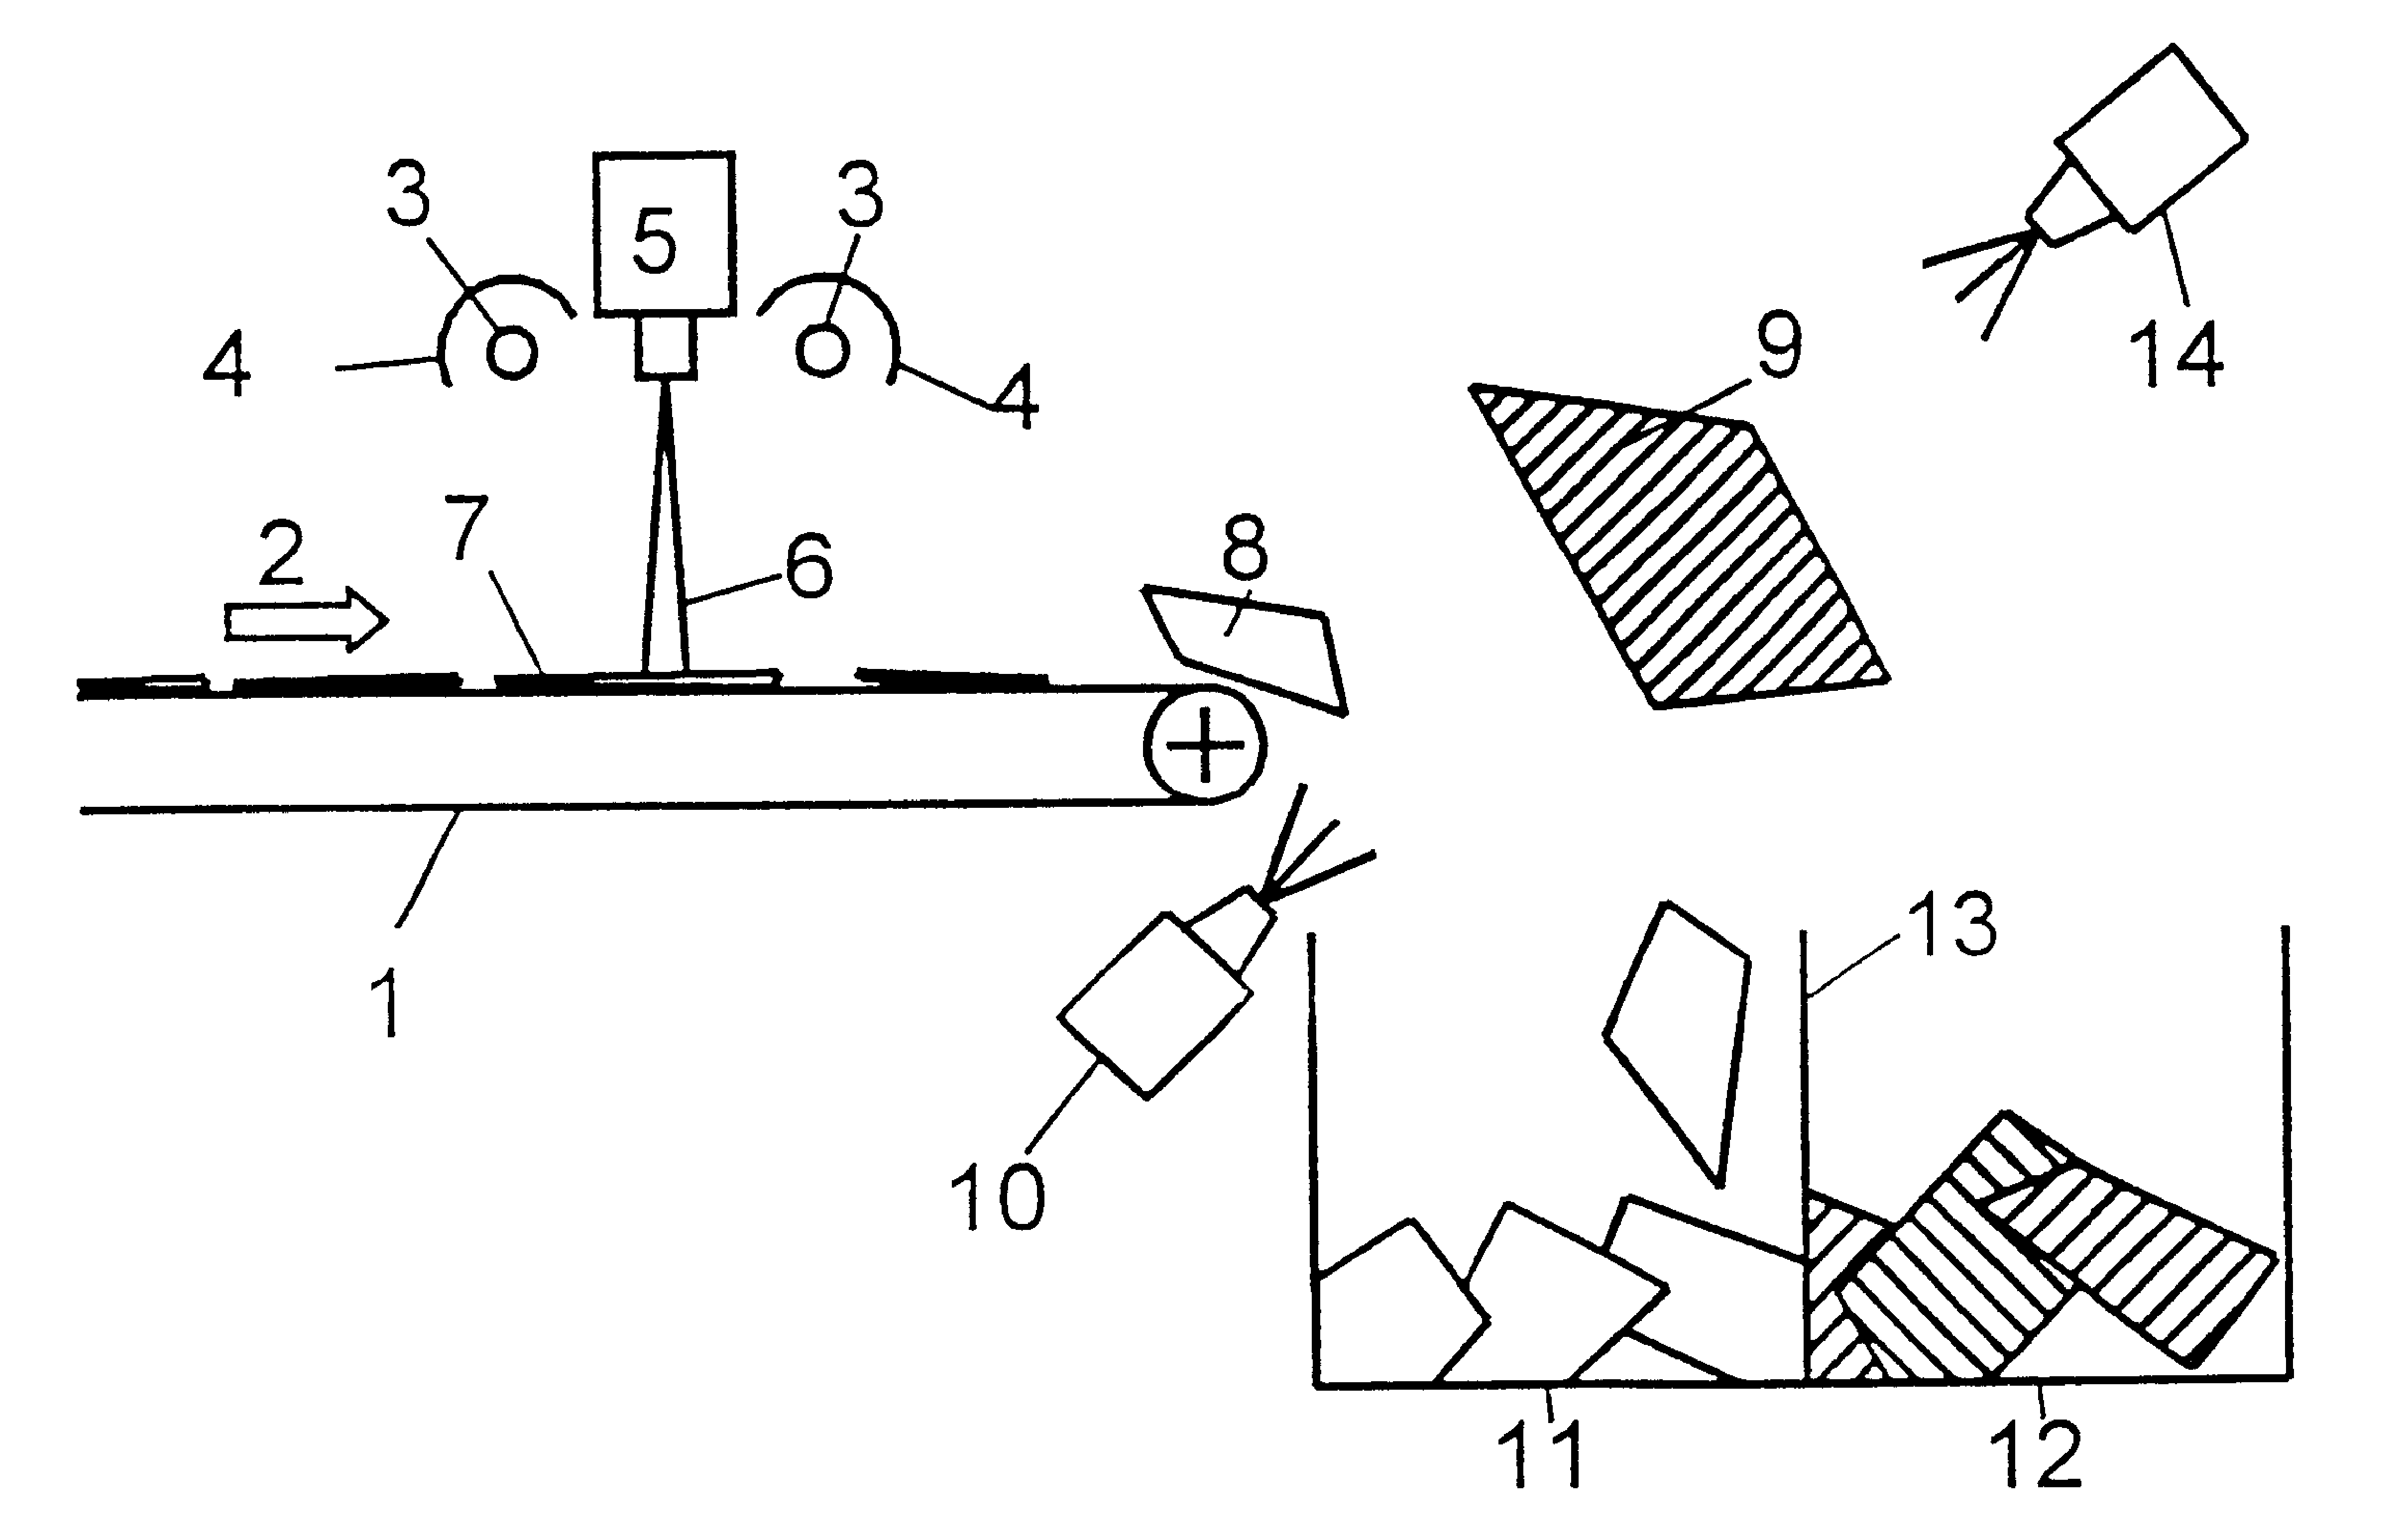
\includegraphics[width=0.60\textwidth]{eixelberger}
  \par}
  \caption{Scheme of apparatus for sorting waste paper
           of different grades and conditions~\cite{Eixelberger:2003}.}
  \label{afig:eixelberger}
\end{figure}

In 1999, Gschweitl \cite{Gschweitl:1999} patented sorting system that uses
combination of visible light, ultraviolet light, x-rays and/or
infrared light to illuminate the paper for sorting. However,
Gschweitl utilized mechanical system for picking paper which
results in serious performance restrictions.

While definitely being a serious improvement in terms
of high-volume recycling, mentioned methods still lack
of reliability, rather complex, expensive and cannot process
more than two types of paper at a time. In addition, feature extraction
was performed without usage of image processing and
intelligence techniques.

\subsubsection*{ Template Matching Based Waste Paper Sorting System Description }

In the work of MO Rahman et al.~\cite{Rahman:2009} the papers sorting
system based on electronic image. The method is based based on
selection of four supporting points on the image and extracting
features around these points. However, during extraction
procedure no information about the texture of the object
is used what can lead to wrong assumption about the paper
grade. Hence, the main goal of the work presented by
Rahman et al.~\cite{Rahman:2009} is to separate different
types of paper utilizing algorithm of template
matching~\cite{Pham:2003}. In developed system authors
use RGB channels of the paper sample image to
construct RGBString for N-cell to overcome an issue
with previously developed system.

As can be seen from block diagram presented on Figure~\ref{afig:tempmatch}
the system consist of two main modules, namely identification module
and enrollment module. Both of these phases share some of the steps.
Every module starts with image acquisition, preprocessing,
and feature extraction. The enrollment phase continues with construction
of RGBString for initialization of reference database.
The indention phase continues with RGBString construction
for N-cells, matching, and decision.

\begin{figure}[htp]
  {\par\centering
  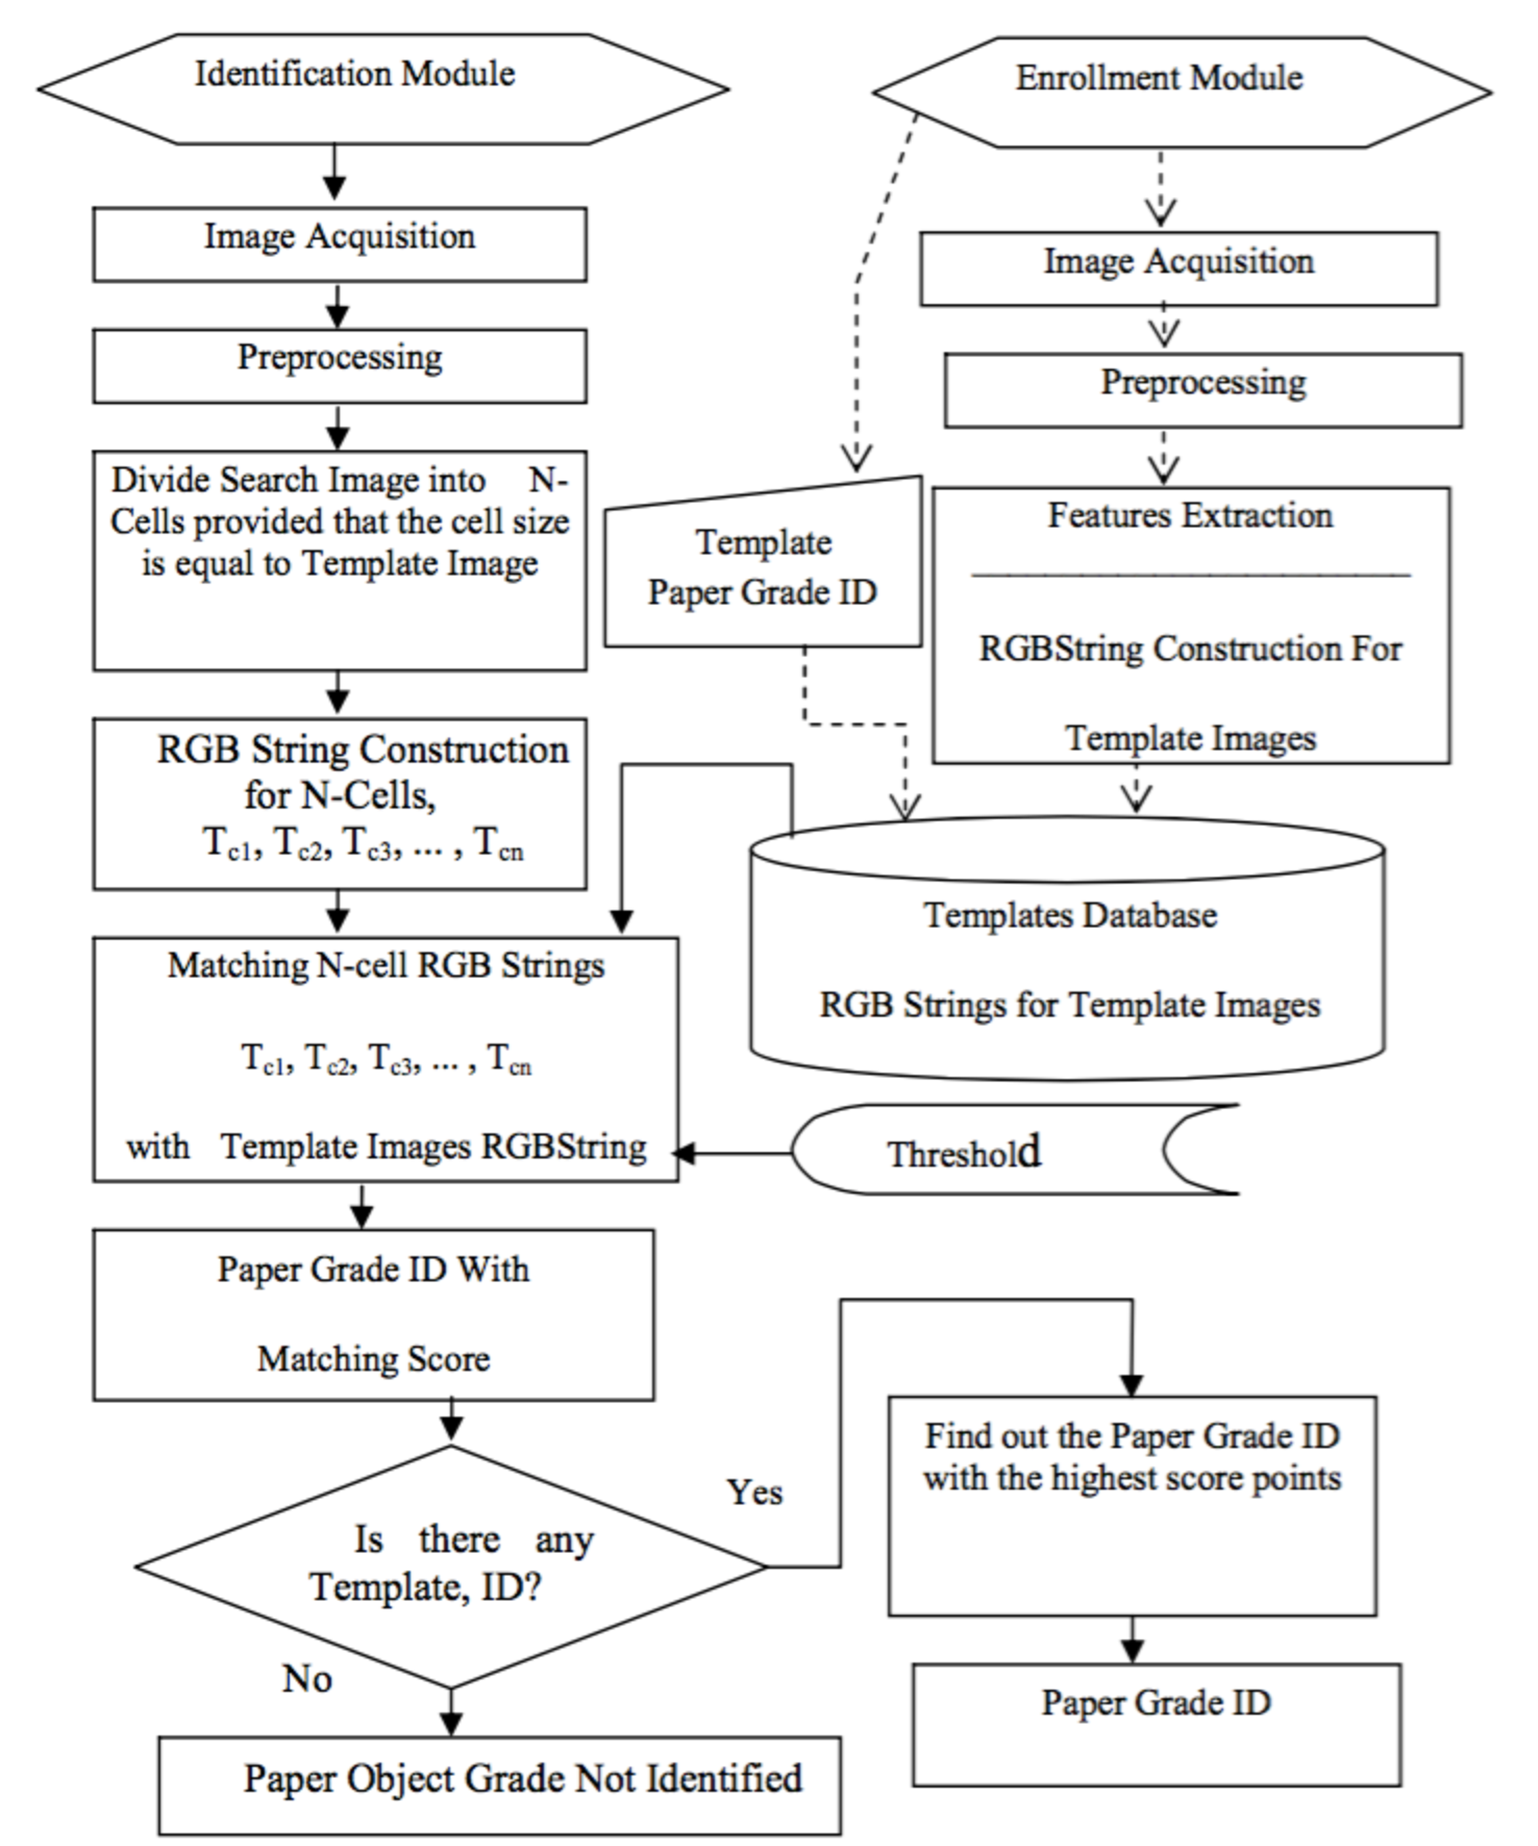
\includegraphics[width=1\textwidth]{tempmatch}
  \par}
  \caption{Block Diagram of the Paper Grade Identification
          System Using Template Matching~\cite{Rahman:2009}}
  \label{afig:tempmatch}
\end{figure}

The size of the taken images in describing system is $320\times240$. Images
taken by common webcam in the RGB mode. The webcam's settings such as
the brightness, contrast and saturation are set to 50\%, 50\%, 100\%
accordingly. It was revealed that performance strictly depends on
quality of illumination. Once calibration was done, for this
experiment authors chose front lighting-directional-darkfield
illumination \cite{Pham:2003}. The speed of the conveyor belt
was set to 14 feet per minute. In course of scanning, system
generates two types of signals, such as presence of object (PObj) and
absence of object (AObj). Those two signals are used to properly
handle separation of objects on conveyor belt in such manner that if presence
signal is followed by absence signal then camera is making a photo
of inspected zone.

The image preprocessing is done after making a
photo of inspection zone a trimming unnecessary boundaries. Once
this step is performed, the next action is to remove
background noise by applying the combination
of thresholding and morphological operation
erosion using $3\times3$ convolution filter.

The paper image uses 3 channels for its representation,
namely $R$ (red), $G$ (green) and $B$ (blue). To obtain gray scale
image standard transformation is performed~(\ref{eq:rgb}).

\begin{equation}\label{eq:rgb}
  Y = \frac{R \times G \times B}{3}
\end{equation}

The $Y$ component is named this way to avoid collisions with green channel.
To construct RGB string authors use maximum of 3 color channels
as first part of RGBString, then second channel and finally
channel with lowest value. The $Y$ channel has reserved
fourth place in RGBString. The frequency of appearance
of the certain color component is related to its value,
because ranges of values for different components are
distinct for different types of paper. The color repetition
process is described by Listing~\ref{lst:colorrep}.

\begin{lstlisting}[caption={Color Repetiotion Calculation}, label={lst:colorep}]
# Color repetition in RGBString

if color_value <= 63: color_repetition = 1
elif color_value <= 184: color_repetition = 2
elif color_value <= 229: color_repetition = 3
else: color_repetition = 4
\end{lstlisting}

To construct template, the system obtains the information
related to region of interest and RGBString
after getting template width (TW) and template height (TH)
values of the template image. As it illustrated on figure~\ref{afig:searchimg}, the
search image is partitioned into N-cells. The cell
image should have equal size to template image.
All of the redundant cells are filtered beforehand.

\begin{figure}[htp]
  {\par\centering
  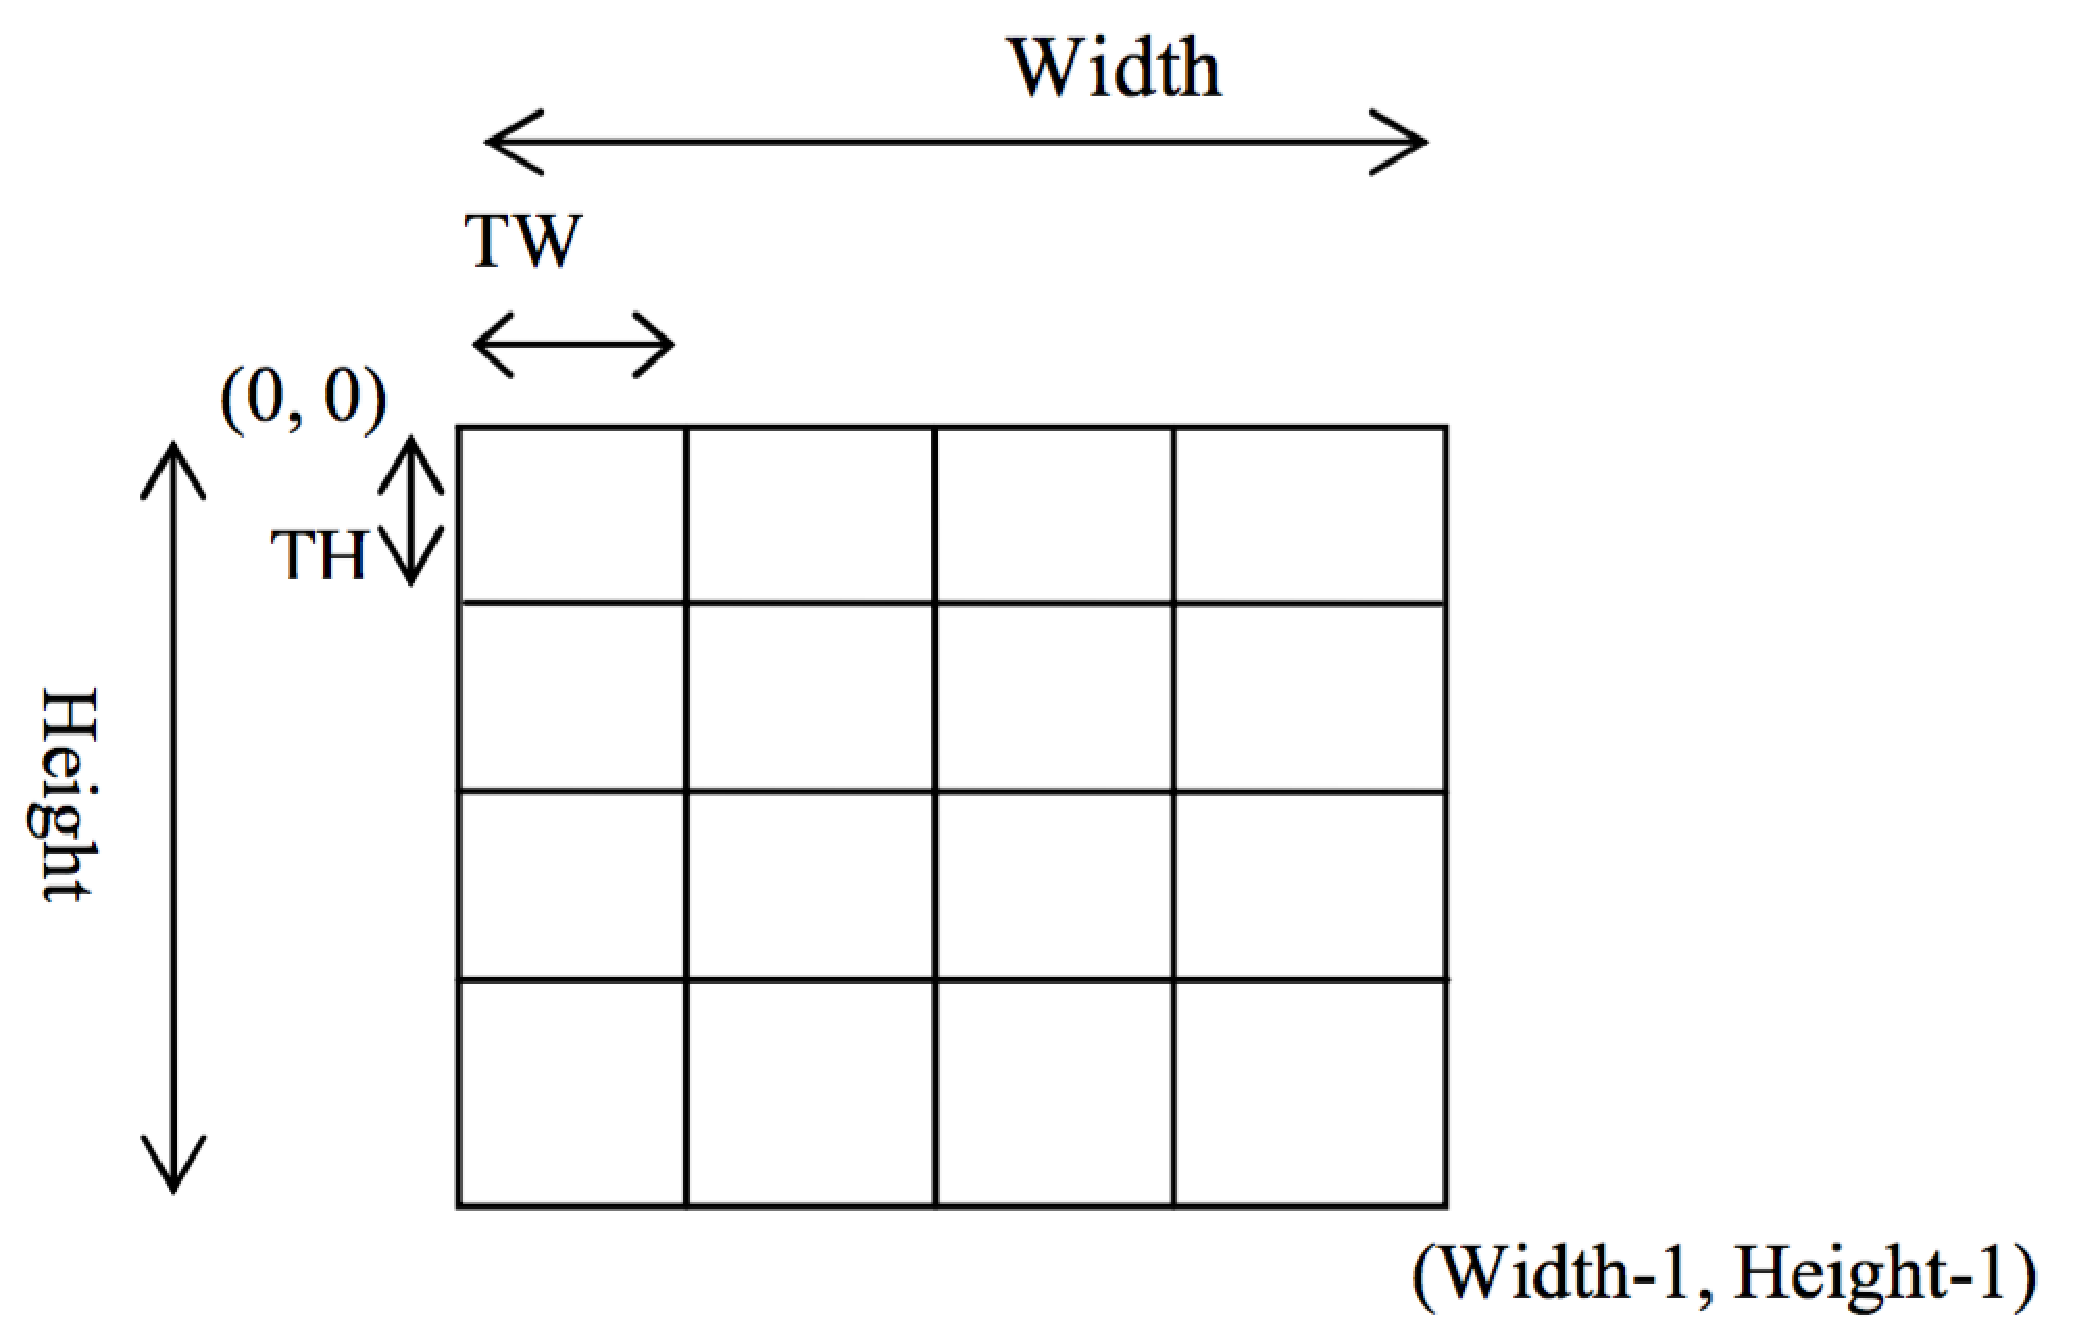
\includegraphics[width=0.55\textwidth]{searchimg}
  \par}
  \caption{Search Image and Template Image~\cite{Rahman:2009}}
  \label{afig:searchimg}
\end{figure}

The core idea of the template matching procedure is based
on string matching algorithm. The process can be described
as follows. For every template image and
every cell from the grid the matching score is calculated
using string matching. If the score is greater than
threshold then template is increased by one (Listing~\ref{lst:tempmatch}).
For their implementation authors use
92\% as threshold value.

\begin{lstlisting}[caption={Template Matching Procedure}, label={lst:tempmatch}]
# Template matching
for template in templates:
    for cell in cells(image):
        score = compare_rgbstrings(template, cell)
        if score >= threshold:
            templateOccurance[template] += 1
\end{lstlisting}

Once matching process is finished, the next step is decision
making. In this procedure, templates are iterated
one by one retrieving occurrence, if occurrence of the certain
template is higher than others then paper is graded by the
index of this template.

\begin{lstlisting}[caption={Decision Making Procedure}, label={lst:decision}]
# Decision making
tmax = 0
length = len(templates) # number of templates
papergrade = 1
for i in range(1,length):
    if templateOccurance[template] > tmax:
        tmax = templateOccurance[i]
        papergrade = i
\end{lstlisting}

\subsubsection*{ Results }
The authors used three types of paper for testing
purposes, namely Old Corrugated Cardboard (OCC),
Old News Paper (ONP) and White Paper (WP). Those
types are chosen for testing purposes because of
their often occurrence in usual tasks. For experiments
authors selected one hundred paper samples per grade.

The paper object is constructed from
three color channels, this model is able to describe
over 16 millions colors. From the experimental points
of view OCC, ONP, WP colors are fully distinctive,
although for subtractive printing model cyan, magenta,
yellow, and black colors are used. Due to this peculiarity,
not all paper samples use the same color configuration
and it was harder to distinguish deferent paper objects.
In presented experiment, authors used not only different
templates for each type of paper, but also different template
for each size of the same paper grade. The performance
of the system is inversely proportional to the template
size. Thus, the less template size then bigger number of
image cells should be considered which results
in greater computational time.


\begin{table}[hpt]
\begin{center}
\caption{Experiment resutls~\cite{Rahman:2009}.\label{tab:exper}}
{\renewcommand{\arraystretch}{2}
\begin{tabular}{|p{0.25\linewidth}|p{0.2\linewidth}|p{0.2\linewidth}|p{0.2\linewidth}|}

% Title
\hline
\textbf{Method}
&
\textbf{Template Size}
&
\textbf{Name of the Paper Grade}
&
\textbf{Correct Identification Rate} \\
\hline

% Row
\multirow{9}{*}{Template Matching}
&
\multirow{3}{*}{$5\times5$}
& WP & 96\% \\
\cline{3-4}

&& ONP & 92\% \\
\cline{3-4}

&& OCC & 96\% \\
\cline{2-4}

& \multirow{3}{*}{$10\times10$}
& WP & 86\% \\
\cline{3-4}

&& ONP & 82\% \\
\cline{3-4}

&& OCC & 84\% \\
\cline{2-4}

& \multirow{3}{*}{$20\times20$}
& WP & 78\% \\
\cline{3-4}

&& ONP & 72\% \\
\cline{3-4}

&& OCC & 76\% \\
\hline

\end{tabular}}
\end{center}
\end{table}

The success rate of the developed algorithm is presented on Table~\ref{tab:exper}. The
rate has been calculated as ratio between correctly classified paper grades and
misclassified grades. The best result achieved using $5 \times 5$ template size which
is 96\% for WP, 92\% for ONP, and 96\% for OCC.

% ---
% Sorting systems of recyclable materials
% ---
\section{ CONCLUSION }
The problem of separating different kinds of recyclable waste have
received considerable attention. In this work we summarized
the knowledge about the application of machine vision systems which
help to sort such materials as paper and plastic. The key aspects and
possible problems were discussed. The arguments why
manual sorting systems can not be used in industry were stated. The results
of modern algorithm were also presented. The pluses and minuses
of the methods were outlined.

% Bibliography
\addcontentsline{toc}{section}{REFERENCES}
\bibliography{resources/report}

\end{document}
